%==============================================================================%
% SERIALIZABILITY & LOCKING                                                    %
%==============================================================================%

\section{Serializability \& Locking}
...

\begin{multicols}{2}
    \begin{figure}[H]
        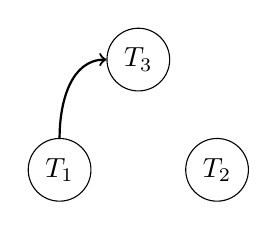
\begin{tikzpicture}
        [
            task/.style={circle, draw},
        ]
            \node[task] (T1) at (0.0, 0.0) {$T_1$};
            \node[task] (T2) at (2.0, 0.0) {$T_2$};
            \node[task] (T3) at (1.0, 1.4) {$T_3$};
            
            \draw[->, thick, draw] (T1.north) to [out=90,in=180] (T3.west);
        \end{tikzpicture}
        \caption{Precedence graph for transaction schedule 1}
        \label{fig:trans-schedule-1}
    \end{figure}

    \colbreak
    
    % TODO: copy/paste
\end{multicols}
